\documentclass{minmal}
\usepackage[utf8]{inputenc}
\usepackage{amsmath, amssymb}
\usepackage{array}
\usepackage{placeins}
\usepackage[colorlinks=true, linkcolor=black, urlcolor=blue]{hyperref}
\usepackage{geometry}  % for marginer
\usepackage{tabularx}  % automatisk kolonnebredde
\geometry{margin=2cm}
\usepackage{caption}
\usepackage{float}
\usepackage{tikz, pgfplots}
\pgfplotsset{compat=1.18}
\usetikzlibrary{decorations.pathreplacing} 
\title{Lambda-metoden ($\lambda$-tuning) for PI-regulatorer\nl[2]
    \centering
    
\includegraphics[width=1\linewidth]{anlegg.png}
\vspace{2cm}
}

\newpage
\date{\today}
\author{Svein-Tore Narvestad}
\begin{document}
\maketitle
\thispagestyle{empty}
\newpage
\tableofcontents
\newpage
\section{Introduksjon}
Når man arbeider med styresystemer i industrien så er det viktig at man har regulatorer med gode regulatorparametre ($K_p$,$T_i$ og $T_d$).  Har man gode parametre kan en regulering se slik ut:

\begin{figure}[h]
    \centering
    
\includegraphics[width=0.5\linewidth]{simc_sim.png}
    \caption{Enter Caption}
    \label{fig:placeholder}
\end{figure}
Men om vi har feil parametre så kan det bli veldig feil.  Her kan du se et eksempel på det:\\

\begin{figure}[h]
    \centering
    
\includegraphics[width=0.5\linewidth]{prosessfag/bilder/regulator_kaos.png}
    \label{fig:placeholder}
\end{figure}


\noindent Vi har tidligere sett på hvordan vi kan optimalisere en prosess med Ziegler-Nichols metode.  Denne gir gode resultater men kan være litt aggressiv.  Men det å øke $K_P$ verdien til man får stående svingninger er noe man sjeldent får til. I hvert fall i virkelige prosessanlegg, som vi skal jobbe med nå.  Et alternativ til denne er Lambda metoden. Lambda-metoden (også kjent som Skogestad-metoden) er en modellbasert metode for å stille inn PI- og PID-regulatorer. Metoden er spesielt nyttig for industrielle prosesser som kan beskrives som førsteordens prosess med dødtid (FOPDT), for eksempel tankanlegg, temperatur- strømnings-mengde- eller nivåprosesser.  
\newpage
\section{Hva er et FOPDT system?}
\subsection{En enkel tankmodell som et FOPDT system}
Vi skal nå se nærmere på hva som menes med et FOPDT system.  Det står for førsteordens prosess med dødtid.  Men hva betyr det?  Et eksempel kan være en tankprosess som vist i figuren under: 
\begin{figure}[h]
    \centering
    
\includegraphics[width=0.7\linewidth]{tankprosess_ny.png}
    \caption{En enkel tankprosess.}
    \label{fig:placeholder}
\end{figure}\\
Vi tenker at vi har en situasjon der det strømmer like mye inn og ut av tanken.  Da vil selvfølgelig nivået i tanken være konstant.  Men om vi åpner opp litt mer på ventilen inn i tanken så vil nivået i tanken stige.  Siden vi har en åpen tank så vil væskemengden ut av tanken også øke.  Det spesielle som skjer da, for et FOPDT system, er at etter en stund vil væskemengden ut av tanken bli lik væskemengden inn i tanken, og nivået vil stabilisere seg igjen.  Dette forløpet kan vi fremstille grafisk:        
\begin{figure}[h]
\centering
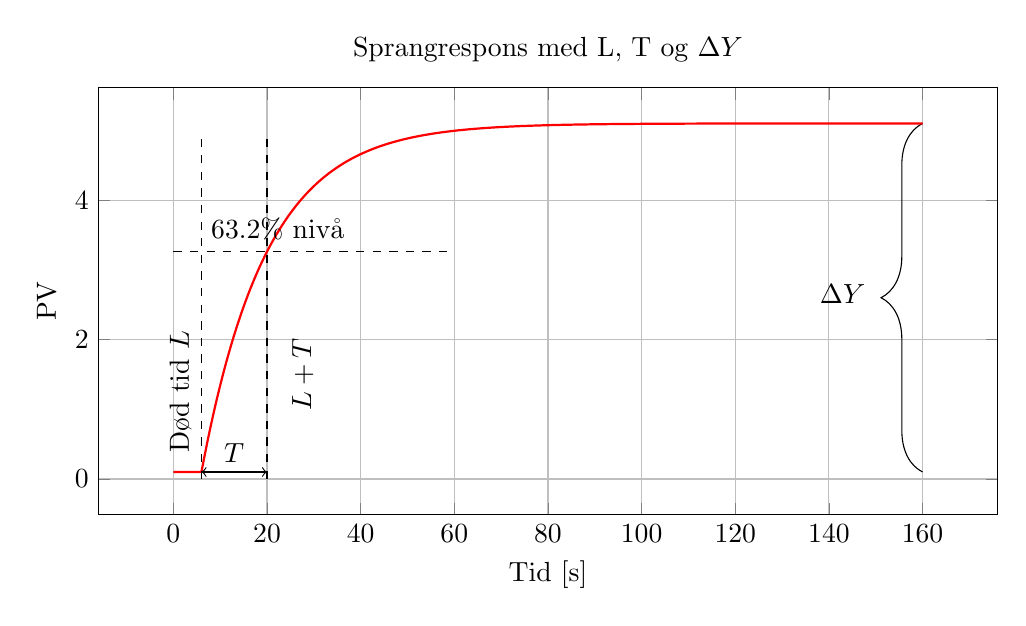
\begin{tikzpicture}

\begin{axis}[
    width=13cm,
    height=7cm,
    xlabel={Tid [s]},
    ylabel={PV},
    grid=both,
    title={Sprangrespons med L, T og $\Delta Y  $},
]

% ] 
--- Parameters ---
\def\L{6}
\def\T{14}
\def\K{1}
\def\dY{5}
\def\Y{0.1}
\def\domain{160}
\draw [decorate, decoration={brace,amplitude=15pt}] (\domain,\Y) -- (\domain,\Y+\dY);
% --- FOPDT response curve ---
\addplot[
    thick,
    red,
    domain=0:\domain,
    samples=400,
]
{ (x < \L) *\Y + (x >= \L) *((1 - exp(-(x-\L)/\T))*\dY+\Y)};

% --- Mark L ---
\addplot[dashed] coordinates {(\L,0) (\L,1*\dY)};
\node[rotate=90, anchor=south] at (axis cs:\L,0.25*\dY) {Død tid $L$};

% --- Mark L+T ---
\pgfmathsetmacro{\LT}{\L + \T}
\addplot[dashed] coordinates {(\LT,0) (\LT,1*\dY)};
\node[rotate=90, anchor=south] at (axis cs:\LT*1.6,0.3*\dY) {$L + T$};

% --- 63.2% line ---
\pgfmathsetmacro{\ytau}{0.632*\dY)+\Y}
\addplot[dashed] coordinates {(0,\ytau) (60,\ytau)};
\node[anchor=west] at (axis cs:1*\L,\ytau*1.1) {63.2\% nivå};

% --- ΔPV marking ---
\node[anchor=west] at (axis cs:\domain*0.85,0.53*\dY) {$\Delta Y$};
\draw[<->]
    (axis cs:\L,\Y)
    --
    (axis cs:\LT,\Y)
    node[midway, above] {$T$};
\end{axis}
\end{tikzpicture}
\end{figure}\\
Her er det noen parametre og måleverdier som er for å beskrive dette FOPDT systemet:
\begin{itemize}
    \item \textit{L}: Dette er dødtiden til prosessen.  Dødtid er tiden fra det skjer en endring i ventilen, og til vi ser en endring i prosessverdien (i dette tilfellet nivået i tanken).  Dødtiden i dette tilfellet er tiden det tar for væsken (den nye væskemengden) å renne ut av ventilen, gjennom røret, og faktisk treffe væskeoverflaten i tanken.   Tiden nivåmåleren (f.eks. en trykktransmitter eller en radarsensor) bruker på å registrere at overflaten faktisk har flyttet på seg vi også være en del av dødtiden.  Så hvor langt røret fra ventil og til tanken er, det er avgjørende for dødtiden i dette tilfellet.  
    \item \textit{$\Delta Y$}: Dette er den totale endringen i prosessverdien (nivået) fra startverdien til den nye stasjonærverdien.  
    \item\textit{$\Delta U$:}Dette er sprangendringen vi ønsker å gjøre manuelt med pådragsorganet, og i dette programmet angis den i prosent.
    \item\textit{K:} Forsterkningen (\(K\)) er forholdet mellom endringen i prosessverdien ($\Delta Y$) og den manuelle endringen i  pådragsorganet ($\Delta U$).   Her er den matematiske definisjonen:\\
    
    \[K=\frac{\Delta Y}{\Delta U}\]
    \item \textit{T}: Tiden etter dødtiden og frem til prosessverdien har nådd 63,2\% av den totale endringen i prosessverdien (63,2\% av $\Delta Y$).
    \item \textit{$Y_0$}: Dette er prosessverdien før sprangendringen. 
    \item \textit{$Y_\infty$}: Dette er prosessverdien når den har nådd en ny stasjonærverdi (en verdi som ikke endrer seg).  Vi ser at vi bruker symbolet $\infty$.  Dette er tegnet for uendelig , og skal vise til at vi har kommet til en ny verdi som ikke endrer seg.  
\end{itemize}
Her er det også viktig å være klar over at $\Delta Y=Y_\infty - Y_0$.  Symbolet $\Delta$ er den greske bokstaven for D.  Og den brukes for forskjeller, for det kalles for \textbf{\textit{D}}ifferanse. Vær klar over at $\Delta Y$ alltid skal oppgis som en positiv verdi i bergnigen våre, selv om $Y_\infty$ er mindre enn $Y_0$.  
\subsection{Et eksempel fra et virkelig tankanlegg}
Vi skal nå se på et mer konkret eksempel på en førsteordens prosess med dødtid.  Dette eksempelet er hentet fra ett av prosessanleggene vi har i klasserommet:  
\begin{figure}[h]
    \centering
    
\includegraphics[width=1.0\linewidth]{sprangresons_uten_regulator.png}
    \caption{nivåets endring når vi gjør en sprangendring}
    \label{fig:placeholder}
\end{figure}\\
Her kommer en forklaring på denne grafen:\\\\
\liste[*]{
\item Etter 38s gjør vi en sprangendring i pådraget på 5\%.  Det tar  ca. 15s fra ventilen får beskjed om å endre seg (5\%) og til nivået begynner å stige .  Denne tiden kaller vi dødtiden L.  Den er merket lilla på grafen (avstanden mellom den røde og lilla er liten, men tilsvarer 15 s).
%Men endringen i pådraget skjer momentant:\\
%\begin{figure}[h]
%    \centering
%    
\includegraphics[width=1.0\linewidth]{sprangendrin_5prosent.png}
%    \caption{Her gjør vi en varig endring i pådraget på 5\%}
%    \label{fig:placeholder}
%\end{figure}\\
\item I grafen under skal vi legge merke til tiden T=422,0s.  Dette er tiden det tar prosessverdien vår ( i dette tilfellet nivået) å nå 63,2\% av sin totale endring.  Vi skal nå forklare hva som menes med SIMC metoden.  Det handler om at regulatoren, med sine PID parametre, klarer å styre prosessen vår som en FOPDT prosess men med en tidskonstant som er mindre enn selve prosessen.  Tidskonstanten for FOPDT prosessen til regulatoren kaller vi lambda ($\lambda$).  I grafen under ser vi regulatoren når den har en tidskonstant $\lambda$ som er halvparten av tidskonstanten til prosessen:\\
\begin{figure}[h]
    \centering
    
\includegraphics[width=1\linewidth]{regulator_med_lambda_2.png}
    \caption{Denne figuren viser fint hvordan $\lambda$ regulering fungerer.}
    \label{fig:placeholder}
\end{figure}\\
Denne figuren viser fint hvordan $\lambda$ regulering fungerer. Når vi halverer tidskonstanten ($\lambda=T/2$) oppnår prosessen det nye set-punktet på halvparten av tiden.}
\newpage
Hva vil skje om vi halverer $\lambda$ verdien en gang til, altså setter $\lambda=T/4$?  Det ser vi grafen:\\
\begin{figure}[h]
    \centering
    
\includegraphics[width=1\linewidth]{prosessfag//produksjonsfaget/lambdaT_4.png}
    \caption{Her ser vi hvordan reguleringen blir når $\lambda=T/4$.   Vi legge rmerke til at reguleringen har nådd 98,2\% på den tiden prosessen uten regulering har nådd 63,2\%.} 
    \label{fig:placeholder}
\end{figure}\nl[1]
Vi ser at vi med $\lambda=T/4=422s/4=105,4s$ så vil prosessen oppnå 98,2\% etter $4\cdot\lambda=4\cdot105,5s=422s$\footnote{En FOPDT prosess når 98,2\% når det har gått tiden $4\cdot T$ etter dødtiden L.  Når du har en regulator når den 98,2\% når det har gått tiden $4\cdot\lambda$ etter dødtiden L.  Man velger ofte å se på dette som den nye stasjonærverdien, for man er veldig nær 100\%.}.  Det betyr at når $\lambda=T/4=422s/4=105,5s$  så vil prosessen  vår nå ny stasjonærverdi på den tiden prosessen utgen regulering bruker på å nå 63,2\% av ny stasjonærverdi.  Prosessen går m.a.o. 4 ganger så raskt. Når vi ser på disse kurvene så er det to momenter som viser at SIMC metoden er god:\\
\liste[*] {
    \item PI regulatoren vil gi oss en respons som følger en førsteordens prosess med dødtid. Tidskonstanten vil være lik $\lambda$. Dette gir oss en veldig stabil regulering.
    \item Ved å endre $\lambda$ verdien kan vi praktisk talt bestemme hvor rask prosessen skal være uten at vi får ustabilitet (mye svinginger) og oversving. 
    }
\subsection{Formler for beregning av PI-parametre}
Vi skal nå se på hvordan vi skal  beregne regulatorparameterne $K_P$ og integraltiden $T_i$ .  Først beregnes prosessforsterkningen  $K$:\\\\
\begin{center}
        {\Large $K=\frac{\Delta Y}{\Delta U}$}
\end{center}\nl[2]
\newpage
\noindent \textbf{Valg av lukket sløyfe-tidskonstant (\texorpdfstring{$\lambda$}{lambda})}:\\\\
Så må vi velge $\lambda$ avhengig av den robusthet og respons vi ønsker:
\[
\lambda = T/2 \quad (\text{rolig, stabil})
\]
\[
\lambda = T/4 \quad (\text{moderat, robust})
\]
\[ 
\lambda = T/6 \quad (\text{rask respons})
\]

Så beregnes parametrene $(K_P \: og \: T_I)$ for en PI-regulator:
\begin{equation}
K_p = \frac{T}{K (\lambda + L)}
\end{equation}
\begin{equation}
T_i = min(T,4\cdot (\lambda+L))
\end{equation}

\subsection{Beregningseksempel}
I grafen under har vi et eksempel fra en nivåprosess:\\
\begin{figure}[h]
    \centering
    
\includegraphics[width=1\linewidth]{sprangresons_uten_regulator.png}
    \caption{Et eksempel for en nivåprosees}
    \label{fig:placeholder}
\end{figure}\\
Her ser vi at:

\[
\Delta Y= 65,0, \quad T = 422,0s\quad L = 15,0s \quad Y_0=11,3\%
\]
Vi kan velge:  \[\lambda = \frac{T}{2}=\frac{422,0s}{2}=211,0s\].

Så må vi beregne K (sprangendring $\Delta U=5\%$) :\\

\[K=\frac{\Delta Y}{\Delta U}=\frac{54,0\%}{5\%}=13,0\]
\newpage
Da blir PI-parametrene:\\\\

\begin{align}
K_p=\frac{T}{K\cdot(\lambda+L)}=\frac{422,0s}{13,0 \cdot (211,0s + 15)s}=0,14
\end{align}
\noindent For $T_i$ får vi:\\\\
$T_i =min(T,4\cdot(\lambda+L))=min(125,40s,4\cdot(211,0+15)s)$\\\\
$T_i=min(422,0\:s,904,0\:s)$\\\\

\noindent $422,0\:s$ er mindre enn $904,0\:s$. Dermed blir $T_i=422,0\:s$. 
Dette gir en stabil og rolig regulering, egnet for tankprosesser. 
Tabellen under gir en oversikt over hvordan man skal beregne regulatorparametrene:
\begin{table}[h!]
\centering
\small
\caption{SIMC-tuning for FOPDT: PI og PID}
\begin{tabular}{|l|m{2cm}|m{4cm}|m{1cm}|>{\raggedright\arraybackslash}m{4cm}|}
\hline
\textbf{Regulator} & \(\mathbf{K_p}\) & \(\mathbf{T_i}\) & \(\mathbf{T_d}\) & \textbf{Kommentar} \\
\hline
PI (offisiell SIMC) & 
\(\displaystyle\frac{T}{k(\lambda+L)}\) & 
 $T_i = min(T,4\cdot (\lambda+L))$& 
-- & 
Standard SIMC for nivå/tank; anbefalt for de fleste FOPDT-prosesser. \\
\hline
PID (praktisk FOPDT-variant) & 
\(\displaystyle \frac{T}{k(\lambda + L/2)}\) & 
\(T\) & 
\(L/2\) & 
Brukes når man ønsker PID selv om prosessen er FOPDT. Mild derivatvirkning for å kompensere dødtid. \\
\hline

\end{tabular}

\vspace{2mm}
\footnotesize
\textbf{Merk:} Mindre \(\lambda\) gir raskere respons, større \(\lambda\) gir mer robust regulering.
\end{table}
\newpage
\section{Fremgangsmåte for Lambda-tuning} 
 Vi skal nå utføre en lambda tuning med simulartoren vi har.  Denne har følgende skjermbilde:
 \begin{figure}[h]
     \centering
     
\includegraphics[width=1\linewidth]{simulator_bilde.png}
     \caption{Dette er skjermbildet til simuleringsprogrammet vårt.}
 \end{figure}\\
 I dette skjermbildet er disse områdene viktige:\\
 \begin{figure}[h]
     \centering
     
\includegraphics[width=0.5\linewidth]{sprangendringer.png}
     \caption{Her kan vi velge om vi vil gjøre en sprangendring i pådraget (manuell sprangendring), eller en sprangendring i set punktet.}
 \end{figure}
 \begin{figure}[h]
     \centering
     
\includegraphics[width=0.75\linewidth]{regulator.png}
     \caption{Her ser vi hvordan vi setter regulator parametrene ($K_p$,$T_i$ og $T_d$).  Her setter man også set-punkt (SKAL-verdi) og velger enten Manuell eller Auto. Når man har valgt Manuell styres pådraget med skyve-kontrollen til høyre (0-100\%).}
 \end{figure}
 \newpage
\subsection{gjennomføring av sprangrespons}
I simuleringsprogrammet er det to typer sprangresons vi kan utgføre. Og det er en manuell endring i pådraget (uten regulator) eller en endring SKAL-verdi (med regulator).   Vi må starte med å gjøre en manuell positiv endring i pådraget $\Delta U$ på f.eks. 5--10\%.  Noter denne verdien, og kall den for $\Delta U$.  Dette gjør du på følgende sted på skjermen (styresystemet):\\
\begin{figure}[h]
    \centering
    
\includegraphics[width=0.3\linewidth]{prosessfag/bilder/sprangendring_manuell.png}
    \caption{Trykk på knappen for å gjøre sprangendring}
    \label{fig:placeholder}
\end{figure}\\

Still inn den sprangendringen du ønsker (i \%) og trykk deretter på sprangendring (manuell).\newpage  
NB! Det er viktig at regulatoren er slått av (at den er i manuell) \textbf{før} du gjør dette:\\
\begin{figure}[h]
    \centering
    
\includegraphics[width=0.4\linewidth]{prosessfag/bilder/sett_i_manuell.png}
    \caption{Husk at regulatoren må være i manuell}
    \label{fig:placeholder}
\end{figure}\\

Når du trykker på sprangendring manuell så vil pumpen øke med verdien du har valgt (sånn cirka 5 eller 10\%).  Hvis du vi ha noe annet kan du endre dette med sprangendring(\%) under bryteren, der det står 20. En sprangendring vil selvsagt føre til at nivået i tanken stiger. Men ikke til evig tid. Bare til væskemengden ut av tanken har økt og blitt lik væskemengden som pumpen gir (\textbf{dette er viktig å forstå}). Når nivået stabiliserer seg sier vi at kurven til nivået viser en \textbf{sprangrespons}.  Sprangresponsen viser hvordan nivået responderer på en manuell sprangendring i pådraget. Du skal altså vente til nivået igjen stabiliserer seg (dette kan ta tid, 5-10 min. for denne prosessen).  Når du har nådd ny stasjonær-verdi (altså fått en verdi som ikke endrer seg, eller endrer seg lite) trykker du på lagre (NB! du må holde knappen nede i noen sekunder før den reagerer):
\begin{figure}[h]
    \centering
    
\includegraphics[width=0.5\linewidth]{lagre.png}
    \caption{Hold lagre knappen nede noen sekunder til den reagerer}
    \label{fig:placeholder}
\end{figure}

Etter en kort stund vil du få opp et vindu for å kunne lagre dataene dine:\\
\begin{figure}[h]
    \centering
    
\includegraphics[width=1\linewidth]{prosessfag/bilder/filedialog.png}
    \caption{Skriv inn et filnavn for å lagre dataene dine}
    \label{fig:placeholder}
\end{figure}
\\Så lagrer du dataene på PC'en din.  De skal du bruke til å finne prosessparameterne ($\Delta Y$, T, L og $y_0$)  for prosessen i Colab.\\
\subsection{Identifisering av prosessparametre}
Nå som vi har dataene fra sprangresponsen lagret på PC'en så kan vi gjøre en analyse av dataene i Colab.  Da kan du åpne følgende lenke: \href{https://colab.research.google.com/github/Svein-Tore/colab/blob/main/FOPDT_Interaktiv_Notatbok_undervisning.ipynb}{FOPDT Interaktiv Notatbok for undervisning}.  Når du kommer inn i Colab så får du opp følgende skjermbilde:
\begin{figure}[h]
    \centering
    
\includegraphics[width=0.75\linewidth]{Colab_oppstart.png}
   \caption{Trykk på play-knappen (se rød sirkel) for å starte notatboken}
    \label{fig:placeholder}
\end{figure}\\
Det er ikke så innlysende hva du skal gjøre nå. Men hvis du fører musepekeren over koden så vil det komme frem en svart play knapp (Se rød sirkel figuren over).  Trykk på denne og programmet i notatboken vil starte.  Men først får du opp følgende:

\begin{figure}[h]
    \centering
    
\includegraphics[width=0.75\linewidth]{start_colab_session.png}
    \caption{Dette er bare en advarsel, så her velger du Kjør likevel.}
    \label{fig:placeholder}
\end{figure}
\noindent Denne advarselen behøver du ikke å bry deg om.  Velg Kjør likevel. Så går du nedover på nettsiden til du kommer til en der det står velg filer:
\begin{figure}[h]
    \centering
    
\includegraphics[width=0.75\linewidth]{velg_filer.png}
    \caption{Gå nedover på nettsiden til du finner knappen Velg filer.}
    \label{fig:placeholder}
\end{figure}
\\Når du trykker på Velg filer får du opp en fil-dialog hvor du velger filen du lagret når du utførte sprangresponsen.\newpage
Programmet vil da tegne en graf av sprangresponsen din:
\begin{figure}[h]
    \centering
    
\includegraphics[width=1\linewidth]{sprang_respons_ny.png}
    \caption{blå kurve viser dine måledata.  Rød kurve viser tilpasset FOPDT kurve.}
    \label{fig:placeholder}
\end{figure}\\
Her trengs det litt forklaringer.  Den blå kurven viser måledataene dine som er lagret i filen.  Den røde kurven er en tilpasning til denne kurven\footnote{For spesielt interesserte: denne kurven kan matematisk skrives slik: $y=y_0+\Delta Y\cdot (1-e^{-(\frac{t-L}{T})})$}.  Fra responsen kan du lese av:
\begin{itemize}
    \item \textbf{Dødtid (L):} tidspunktet der prosessverdien (PV) først begynner å endre seg etter sprangendringen i pådraget. I grafen over er L=13,80s.
    \item \textbf{Tidskonstant (T):} tiden det tar for PV (\textbf{P}rosess \textbf{V}erdi) å nå 63,2\% av endringen etter forsinkelsen.  I grafen over er T=117,20s.
    \item startvedi for nivået, $y_0$.  I grafen over er $y_0=11,79\%$.
    \item Endring i nivå ($\Delta Y$). I grafen over er $\Delta Y=28,75\%$
    \item \textbf{Prosessforsterkning (K):} $K=\Delta Y / \Delta U$. Vi har avlest $\Delta Y=28,75\%$.  Du skal ha notert sprangendringen $\Delta U=10\%$.  Da får vi: 
    $$K=\frac{28,75\%}{10\%}=2,88$$
\end{itemize}\newpage
\subsection{Modelltilpasning i Colab}
  Når vi laster filen vår inn i Colab vil den automatisk prøve å beregne $y_0,\: L,\: T\: og\: \Delta Y$.  Disse verdiene er ikke alltid helt optimale.  Spesielt L kan være vanskelig for programmet:\\
  \begin{figure}[h]
      \centering
      
\includegraphics[width=0.25\linewidth]{L_feil_estimat.png}
      \caption{Her ser vi at dødtiden er altfor stor. }
      \label{fig:placeholder}
  \end{figure}\\
  \noindent Vi bruker derfor sliderne for å tilpasse den røde kurven den blå så godt du kan.  Sliderene finner vi til høyre for kurven:
  \begin{figure}[h]
      \centering
      
\includegraphics[width=0.5\linewidth]{sliders.png}
      \caption{Med sliderne kan vi endre de viktige parametrene slik at den røde kurven matcher den blå.}
      \label{fig:placeholder}
  \end{figure}\\
  Endre litt på L slideren for å forstå hva det er du endrer.  \newpage
  Når du er fornøyd ser det noe slikt ut:\\ 
  \begin{figure}[h]
      \centering
      
\includegraphics[width=0.25\linewidth]{slider_L.png}
      \caption{L=5.2 ser ut som en bra verdi}
      \label{fig:placeholder}
  \end{figure}\\
  Juster så de andre parametrene slik at den røde kurven følger den blå så godt som mulig.  Et tips her er at du først tar L og så $y_0$.  Så tar du T og tilslutt $\Delta Y$.  Etter at du har justert $\Delta Y$ så vil muligens T endre seg litt, for de to er avhengige av hverandre. Du må derfor kanskje justere disse litt frem og tilbake.  Når du er fornøyd skriver du ned verdiene dine  for $\Delta Y,\,L\,,T$\, og $y_0$.  Eller du kan trykke på Last ned PNG.  Da får du et bilde av grafen lagret på PC'en.  \newpage Her ser du hva jeg kom frem til:\\
\begin{figure}[h]
    \centering
    
\includegraphics[width=1\linewidth]{FoPDT_final.png}
    \caption{Her har vi tilpasset verdiene så godt vi kan}
    \label{fig:placeholder}
\end{figure}\\
 De ferdige parametrene finner vi nede i høyre hjørne.  Vi ser at dette er en veldig god tilpasning av kurven.
\subsection{Formler for beregning av PI-parametre}
Vi skal nå se på hvordan vi skal  beregne regulatorparameterne $K_P$ og integraltiden $T_i$ .  Først beregnes prosessforsterkningen  $K$:\\\\
\begin{center}
        {\Large $K=\frac{\Delta Y}{\Delta U}$}
\end{center}\nl[2]

\noindent \textbf{Valg av lukket sløyfe-tidskonstant (\texorpdfstring{$\lambda$}{lambda})}:\\\\
Så må vi velge $\lambda$ avhengig av den robusthet og respons vi ønskrer:
\[
\lambda = T/2 \quad (\text{rolig, stabil})
\]
\[
\lambda = T/4 \quad (\text{moderat, robust})
\]
\[ 
\lambda = T/6 \quad (\text{rask respons})
\]

Så beregnes parametrene $(K_P \: og \: T_I)$ for en PI-regulator:
\begin{equation}
K_p = \frac{T}{K (\lambda + L)}
\end{equation}
\begin{equation}
T_i = min(T,4\cdot (\lambda+L))
\end{equation}

\section{Beregningseksempel}
I grafen under har vi et eksempel fra en nivåprosess:\\
\begin{figure}[h]
    \centering
    
\includegraphics[width=1\linewidth]{FoPDT_final.png}
    \caption{Et eksempel for en nivåprosees}
    \label{fig:placeholder}
\end{figure}\\
Her ser vi at:

\[
\Delta Y= 29,04, \quad T = 125,40s\quad L = 5,20s \quad y_0=11,79s
\]
Vi kan velge:  \[\lambda = \frac{T}{2}=\frac{125,40s}{2}=62,7s\].

Så må vi beregne K (sprangendring $\Delta U=10\%$) :\\

\[K=\frac{\Delta Y}{\Delta U}=\frac{29,04\%}{10\%}=2,904\]

Da blir PI-parametrene:\\\\

\begin{align}
K_p=\frac{T}{K\cdot(\lambda+L)}=\frac{125{,}4\,\text{s}}{2,904 \cdot (62{,}7 + 5,2)\,\text{s}}=0,64
\end{align}\newpage
\noindent For $T_i$ får vi:\\\\
$T_i =min(T,4\cdot(\lambda+L))=min(125,40s,4\cdot(62,7+5,2)s)$\\\\
$T_i=min(125,40\:s,271,6\:s)$\\\\

\noindent $125,40\:s$ er mindre enn $271,6\:s$. Dermed blir $T_i=125,40s$. 
Dette gir en stabil og rolig regulering, egnet for tankprosesser. 
Tabellen under gir en oversikt over hvordan man skal beregne regulatorparametrene:
\begin{table}[h!]
\centering
\small
\caption{SIMC-tuning for FOPDT: PI og PID}
\begin{tabular}{|l|m{2cm}|m{4cm}|m{1cm}|>{\raggedright\arraybackslash}m{4cm}|}
\hline
\textbf{Regulator} & \(\mathbf{K_p}\) & \(\mathbf{T_i}\) & \(\mathbf{T_d}\) & \textbf{Kommentar} \\
\hline
PI (offisiell SIMC) & 
\(\displaystyle\frac{T}{k(\lambda+L)}\) & 
 $T_i = min(T,4\cdot (\lambda+L))$& 
-- & 
Standard SIMC for nivå/tank; anbefalt for de fleste FOPDT-prosesser. \\
\hline
PID (praktisk FOPDT-variant) & 
\(\displaystyle \frac{T}{k(\lambda + L/2)}\) & 
\(T\) & 
\(L/2\) & 
Brukes når man ønsker PID selv om prosessen er FOPDT. Mild derivatvirkning for å kompensere dødtid. \\
\hline

\end{tabular}

\vspace{2mm}
\footnotesize
\textbf{Merk:} Mindre \(\lambda\) gir raskere respons, større \(\lambda\) gir mer robust regulering.
\end{table}
\section{Beregning av regulatorparametre med Colab} 
Det å beregne regulatorparametrene er ikke spesielt vanskelig.  Men vi har også utviklet et program som gjør dette veldig enkelt for oss. Vi må da utgangspunkt i en FPODT kurven som vi viste lenger oppe. Den kan se slik ut:
\begin{figure}[h]
    
\includegraphics[width=1\linewidth]{FOPDT_A12_2.png}
    \caption{FOPDT graf for nivåprosess}
    \label{fig:placeholder}
\end{figure}


\noindent Her trenger vi verdiene $K=\Delta  Y/\Delta U=\tfrac{41,44\%}{5\%}=8,29,\ T=151,7s\ L=4,4 ,$\\ $y_0=9,53\% $ og$\  \lambda=T/2=\tfrac{151,7s}{2}=75,85s$.  I tillegg må vi beregne set-punktet til reguleringen. Her trengs det en forklaring.  I FOPDT grafen over ser vi at man startet ved $y_0=9,53\%$, og at man oppnår en ny stasjonærverdi med $\Delta Y=41,44\%$.  Hvis vi skal utføre dette som en regulering så blir  det nye set-punktet:
$$y_{set-punkt}=9,53\%+41,44\%=50,97\%$$
Nå kan vi starte regulator programmet i Colab.  Nettadressen er \href{https://colab.research.google.com/github/Svein-Tore/colab/blob/main/pi_regulator_niva.ipynb}{Regulering av tankanlegg – SIMC og Ziegler–Nichols}.  Programmet ser slik ut, og vi trykker på play-knappen:\\
\begin{figure}[h]
    \centering
    
\includegraphics[width=0.8\linewidth]{regualtor_oppstart.png}
    \caption{Øverst får vi litt informasjon om programmet}
    \label{fig:placeholder}
\end{figure}\\
Etter at vi har trykket på play-knappen så "scroller" vi helt til slutten av koden.  Her må vi vente en stund før vi får frem Velg filer:
\begin{figure}[h]
    \centering
    
\includegraphics[width=0.8\linewidth]{velg_filer.png}
    \caption{Trykk på Velg filer og velg filen du fikk fra FOPDT plottet.}
    \label{fig:placeholder}
\end{figure}
Når du får frem  knappen Velg filer så trykker du på den og velger FOPDT filen din.  Vi får nå opp en graf.   Men den skal vi ikke se på den med det første. Først må vi ordne sliderne  og velge T/2 for $\lambda$ forhold.  Skriv inn verdiene du har fra din FOPDT graf.  For meg  ble det slik:
\begin{figure}[h]
    \centering
    
\includegraphics[width=0.5\linewidth]{PI_parametre_ny.png}
    \caption{Husk at du må skrive punktum (.) og ikke komma (,) for desimaltall}
    \label{fig:placeholder}
\end{figure}
\newpage
Nå skal du få en graf som ligner på denne:
\begin{figure}[h]
    \centering
    
\includegraphics[width=1\linewidth]{FOPDT_REG_NY.png}
    \caption{Denne grønne kurven er FOPDT grafen din.  Den gule er en ideell matematisk regulator med $K_P=0,228,\ og\ T_i=2,53min$.}
    \label{fig:placeholder}
\end{figure}

Hva betyr så disse grafene? Den grønne kurven er dataene fra datafilen din. Den gule er en ideell PI regulator med $\lambda=T/2=75,85s$.   Vi kan enkelt si at regulatorkurven er en FOPDT kurve der tidskonstanten er halvparten av tidskonstanten til  FOPDT grafen.  Det betyr at den når  63,2\% på halvparten av tiden. Så er det også slik at FOPDT prosesser når ca. 98,2\% av full verdi etter 4 ganger tidskonstanten.  Det betyr også at regulatorkurven når ny stasjonærverdi på halvparten av tiden. Oppsummert vil en regulator med $\lambda=T/2$ "jobbe" dobbelt så raskt.   Noe du også kan teste er å sette $\lambda=T=151.7s$. Hvis du gjør det så vil regulatoren være lik FOPDT grafen (eller rettere sagt tilnærmet lik, avhenging av hvor godt den er tilpasset):\\
\begin{figure}[h]
    \centering
    
\includegraphics[width=0.9\linewidth]{FOPDT_LIK_REG_NY.png}
    \caption{Det er ikke så godt å se, men den gule PI regulator kurven ligger bak den grønne.}
    \label{fig:placeholder}
\end{figure}
\\
Det er ikke så godt å se, men den gule PI regulator kurven ligger bak den grønne.  Vi kan o gså sette $\lambda$ lik $T/4=\tfrac{151,7s}{4}=37,93s$.  Da får vi følgende graf:
\begin{figure}[h]
    \centering
    
\includegraphics[width=1\linewidth]{lambda_kvart_ny.png}
    \caption{Her er $\lambda=T/4=37,93s$}
    \label{fig:niva_fig}
\end{figure}\\
Men et interessant spørsmål er om regulatoren vår virkelig vil jobbe dobbelt så raskt med $K_P=0,28,\ og\ T_i=2,93s$.  Det skal vi teste nå.      
\section{Test av regulatorparametre}
Vi skal nå gjøre en ny simulering, men denne gangen med regulator.  Vi legger da inn $K_P$ og $T_i$ inn i regulatoren i prosessanleggets regulator.  For dette tilfellet med $\lambda=T/2$ får vi $K_P=0,228$ og $T_i=2,53min$.  Vi legger inn verdiene i prosessanleggets regulator:\\
\begin{figure}[h]
    \centering
    
\includegraphics[width=0.3\linewidth]{pI_parametre_prosessanlegg.png}
    \caption{Her skriver du inn $K_P$ og $T_i$}
    \label{fig:placeholder}
\end{figure}\newpage
Så må du oppgi SKAL verdi. Den er litt vanskelig å forstå.  Men den må settes lik $y_0=9,53\%$:\\
\begin{figure}[h]
    \centering
    
\includegraphics[width=0.2\linewidth]{Sett_SKAL_Verdi.png}
    \caption{Sett SKAL verdien lik 9,53\%}
    \label{fig:placeholder}
\end{figure}\\
Så må du slå på regualtoren.  Dette gjør du med denne knappen:
\begin{figure}[h]
    \centering
    
\includegraphics[width=0.25\linewidth]{regulatori Auto.png}
    \caption{Husk på at du må sette regulatoren i Auto}
    \label{fig:placeholder}
\end{figure}\\
Så kommer altså den kjedelige jobben.  Du må nå vente til regulatoren klarer å få  nivået opp til 9,53\%.  Dette kan ta litt tid.   Vær klar over at regulatoren ikke nødvendigvis får akkurat denne verdien.  Vi kan si at $\pm 0,25$\% er akseptabelt.  Når den har stabilisert seg kan vi starte en sprangrespons i set punktet.  Det betyr at vi skal endre set-punktet med en bestemt verdi ( men vi skal \textbf{ikke endre} set-punktet med knappen SKAL-verdi (\%), men angi sprangendringen  her:\\
\begin{figure}[h]
    \centering
    
\includegraphics[width=0.25\linewidth]{sprangendring_setpunkt.png}
    \caption{Her skriver du inn sprangendringen i prosent. Trykk på knappen for å starte sprangendringen }
    \label{fig:placeholder}
\end{figure}\\
Så må beregne sprangendringen.  Og den er lik $\Delta y$ fra FOPDT grafen. Der fant vi ut at $\Delta y=41,44\%$.  \newpage 
Vi skriver inn at sprangendringen er lik 41,44\% og trykker på knappen når vi er klar:\\
\begin{figure}[h]
    \centering
    
\includegraphics[width=0.25\linewidth]{skriv_inn_sprangendring.png}
    \caption{Her skriver du inn sprangendringen som er lik $\Delta y=41,44\%$.}
    \label{fig:placeholder}
\end{figure}\\
Så er det nok en gang bare å sette seg ned og vente.  Den nye SKAL-verdien nå blir lik: 
        $$SKAL-verdi + sprangendring=9,53\%+41,44\%=50,97\%$$\\
  Legg merke til at verdien $50,97\%$ stemmer overens med verdien i figur \ref{fig:niva_fig}.  Nok en gang må du vente til du oppnår den nye SKAL verdien.  For dette eksempelet er det $50,97\%$.  For deg er det helt sikkert en annen verdi.  Ventetiden er nå selvsagt halvert.  Men jeg anbefaler deg å vente like lenge som for FOPDT plottet slik at de to grafene  vises likt.  Når du er fornøyd trykker du  på Lagre:\\
  \begin{figure}[h]
      \centering
      
\includegraphics[width=0.5\linewidth]{lagre.png}
      \caption{Trykk på lagre knappen som du ser til venstre i bildet.  Hold den nede i noen sekunder til fildialogen kommer opp.}
      \label{fig:placeholder}
  \end{figure}
  
\noindent Gi simuleringen et navn og trykk på OK. Gå nå inn på \url{https://colab.research.google.com/github/Svein-Tore/colab/blob/main/pi_regulator_niva.ipynb} igjen.  Så starter du programmet (trykk på play knappen). Så må du legge inn alle verdiene du brukte sist. For meg ble det slik:\\
  \begin{figure}[h]
      \centering
      
\includegraphics[width=0.5\linewidth]{PI_parametre_NY.png}
      \caption{Husk å legge inn de riktige parametrene.}
      \label{fig:placeholder}
  \end{figure}\newpage
  Nå må du trykke på  velg filer:\\
  \begin{figure}[h]
      \centering
      
\includegraphics[width=1\linewidth]{velg_filer.png}
      \caption{Trykk på velg filer.}
      \label{fig:placeholder}
  \end{figure}\\
  
  I fildialogen som nå kommer opp skal du velge to filer: FOPDT plottet og reguleringen.  trykk på den første. Så holder du nete CTRL tasten når du skal velge den andre:\\
  \begin{figure}[h]
      \centering
      
\includegraphics[width=1\linewidth]{velg_to_filer.png}
      \caption{Merk filene du vil ha med i plottet.  Hold nede CTRL tasten når du velger flere filer.}
      \label{fig:placeholder}
  \end{figure}\newpage
  
  Så trykker du på Åpne.  Da vil du få et plott  som inneholder 3 grafer:\\
  \begin{figure}[h]
      \centering
      
\includegraphics[width=1\linewidth]{regulator_testing_ny.png}
      \caption{Rød kurve er FOPDT plott, grønn kurve er virkelig regulator (med anlegget) og gul er matematisk regulator.}
      \label{fig:placeholder}
  \end{figure}\\
  Her kommer en liten forklaring på dette viktige plottet:\\
\begin{itemize}
    \item  Den røde kurven er FOPDT plottet du startet med.  Det kommer frem når du gjør en sprangedring i pådraget (på 5\% eller 10\%).  
    \item Basert på verdiene for $K,T$, $\lambda$ og $L$  beregner dataprogrammet $K_P$ og $T_i$ .  Programmet vil så lage den gule kurven, som er en matematisk  modell/simulering av reguleringen.  Vi kan si at denne kurven prøver å forutsi hvordan reguleringen blir med de gitte parametrene.  Litt komplisert sagt, man finner regulatorparametre som vil gi en FODPT "oppførsel" med tidskonstant lik $\lambda$ verdien ($=T/2$ for oss).  Vi får da en regulering som går dobbelt så fort som sprangresponsen uten regulator.
    \item Den grønne kurven er prosessanlegget vårt med en sprangendring i SKAL verdi som vil tilsvare FOPDT plottet (Vi starter med $y_0=9,53\%\;og\;sprangendring\ lik\; \Delta y=41,44\%$).  Her bruker vi regulatorparametrene vi har beregnet ($K_P=0,228,\ T_i=2,53 min$).
\end{itemize}
Vi ser nå at med lambda metoden så kan vi faktisk på en måte bestemme hvordan regulatoren skal jobbe.   Vi vet at regulatoren vil regulere slik at vi får en første ordens prosess med (liten) dødtid.   Og så kan vi bestemme hvor rask og robust  den skal være.  Dette gjør vi ved å sette lambda verdien.  Det er også viktig å få frem at denne kurven er veldig bra.  Her er det godt samsvar mellom det teoretiske (gul kurve) og prosess (grønn kurve).\newpage
Her ser du to andre eksempler for den samme sprangendringen:\\
\begin{figure}[H]
    \centering
    
\includegraphics[width=1\linewidth]{NY_KURVE.png}
    \caption{Her er rød og grønn to reguleringer med anlegget}
    \label{fig:placeholder}
\end{figure}
Her ser vi helt klart at den grønne har noe oversving.  Den røde er klart bedre.  Likevel, ingen av disse to reguleringene kan sies å være dårlige.     

\section {eksempel på sprangresponser}  
Vi skal nå vise noen grafer som viser spesiellle fenomener i sprangresponer.
\subsection{Dødtid:}
Grafen under viser sprangrespons med dødtid (rød) og uten dødtid (blå)   
 \begin{figure}[ht]
\centering
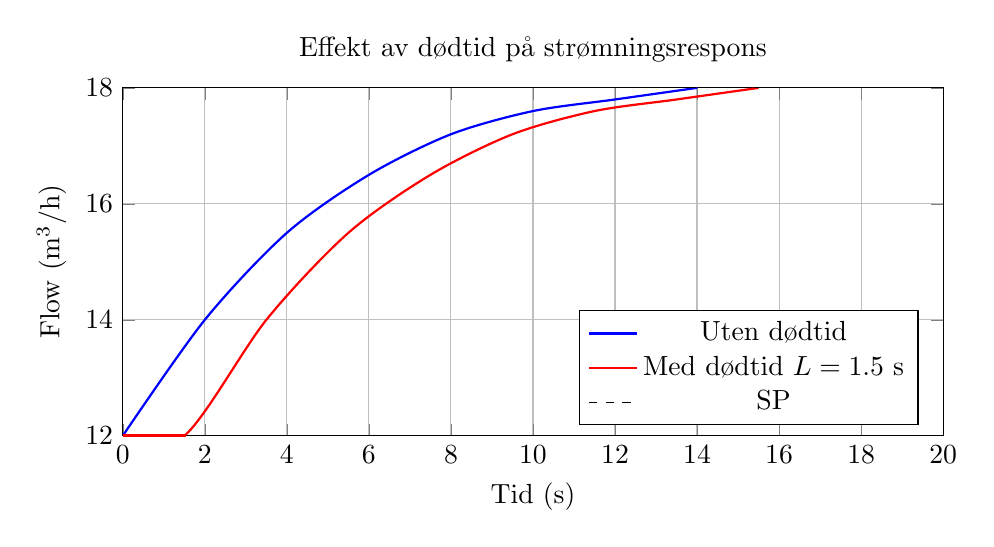
\begin{tikzpicture}
  \begin{axis}[
    width=12cm, height=6cm,
    xlabel=Tid (s),
    ylabel=Flow (m$^3$/h),
    xmin=0, xmax=20,
    ymin=12, ymax=18,
    grid=both,
    legend pos=south east,
    title={Effekt av dødtid på strømningsrespons}
  ]

  % Kurve uten dødtid
  \addplot[thick,blue,smooth] coordinates {
    (0,12.0)
    (2,14.0)
    (4,15.5)
    (6,16.5)
    (8,17.2)
    (10,17.6)
    (12,17.8)
    (14,18.0)
  };
  \addlegendentry{Uten dødtid}

  % Kurve med dødtid L=1.5 s
  \addplot[thick,red,smooth] coordinates {
    (0,12.0)
    (1.5,12.0)
    (3.5,14.0)
    (5.5,15.5)
    (7.5,16.5)
    (9.5,17.2)
    (11.5,17.6)
    (13.5,17.8)
    (15.5,18.0)
  };
  \addlegendentry{Med dødtid $L=1.5$ s}

  % Setpoint linje
  \addplot[dashed,black] coordinates {(0,18) (20,18)};
  \addlegendentry{SP}
  \end{axis}
\draw[red,line width=1.2pt ] (0,0) -- (0.8,0); 
\end{tikzpicture}
\caption{Strømningsprosessen med og uten dødtid. Dødtiden forsinker starten på responsen.}
\end{figure}
\newpage\noindent
\subsection{Hvordan lambda verdien påvirker reguleringen}
Grafen under viser hvordan lambda verdien påvirker reguleringen:
\begin{figure}[h]
    \centering
    
\includegraphics[width=\linewidth]{u_pv_lambda_static.png}
    \caption{Her ser  vi hvordan $\lambda$ verdien vi påvirke reguleringen}
    \label{fig:placeholder}
\end{figure}

Vi ser at lambda metoden som regel sikrer en stabil og robust prosess uten eller med litt oversving.   
\newpage\noindent Men velger vi en veldig lav lambda verdi så kan man få oversving, som vist i grafen under ($\lambda=\frac{T}{10}$):
\begin{figure}[h]
\centering
\begin{tikzpicture}
  \node (img) {
\includegraphics[width=1\linewidth]{ny_T10_50.png}};
  \draw[dashed, thick,blue]
    ([yshift=7.7cm]img.south west) --
    ([yshift=7.7cm]img.south east);
\end{tikzpicture}
\caption{Sprangrespons med veldig lav $\lambda$ verdi}
\end{figure}\\
Men en så lav lambda-verdi anbefales ikke.
\subsection{Pådragsorganets virkemåte}
Om viser på prosessverdiene så ser vi at alle samen ender opp med å nå  SKAL-verdien.  Dette er fordi vi har en PI regulator.  Hadde vi hatt en ren P regulator så hadde vi endt opp med et stasjonæravvik.  Det er også viktig å se på hvordan regulatoren arbeider.
Dette ser vi i det nederste diagrammet:  
\begin{figure}[h]
    \centering
    
\includegraphics[width=0.95\linewidth]{pådra_graf.png}
    \caption{Her ser du hvordan pådragsorganet "jobber"}
    \label{fig:placeholder}
\end{figure}\\
Legg merke til at i starten "hopper" pådraget opp for så å øke lineært for deretter å synke.  Stigningen skjer under dødtiden.  Grunnen til at man ofte ser den lineære stigningen akkurat i dødtiden, er at \textbf{avviket er konstant} mens vi venter på at prosessen skal reagere.\\\\
\textbf{Forklaring:}
\begin{enumerate}
    \item \textbf{Sprang:} Du endrer setpunktet. P-leddet gir et \textbf{hopp}.
    \item \textbf{Dødtid:} Ingenting skjer i prosessen ennå. Avviket er derfor maksimalt og helt flatt.
    \item \textbf{Stigning:} Fordi avviket er konstant og flatt i dødtiden, vil I-leddet summere det opp som en \textbf{perfekt rett linje oppover}.
    \item \textbf{Reaksjon:} Når dødtiden er over og prosessen begynner å bevege seg, blir avviket mindre, og stigningen flater ut eller begynner å synke.
\end{enumerate}
Vi har nå sett på hvordan pådragsorganet arbeider.
\section {kalibrering av nivåmåler}
Når vi kalibrerer en sensor så skal vi ha 4 mA ved nedre måleverdi, og 20mA ved øvre måleverdi. For et nivå har vi:

Nedre måleverdi: 0\% (signal: 4mA)

Øvre måleverdi: 100\% (signal 20mA)\\

\noindent Det som er fint med dP cellene vi har er at vi fritt kan velge hva som er øvre og nedre måleverdi. Vi stiller inn nivået på nedre måleverdi, og setter strømmen til 4mA. Dette gjøres ved å bruke knapper på dP cellen:\\
\begin{figure}[h]
    \centering
    
\includegraphics[width=0.3\linewidth]{kalibrering1.png}
    \caption{Her er du de 3 knappene M,S og Z på dP cellen.}
    \label{fig:placeholder}
\end{figure}\\
Vi har følgende knapper:

M - mode knapp. Denne brukes for å aktivere menyene.

S - Span knapp. Denne bruke vi til å velge de ulike tallene (vi kommer tilbake til dette)

Z - Zero knapp. Denne bruker vi til å endre verdi på tallene.\\

\newpage 
\noindent Vi skal nå gå igjennom kalibreringsrutinen. Vi starter med dP cellen i visingsmodus.\\
Da ser den slik ut:\\
\begin{figure}[h]
    \centering
    
\includegraphics[width=0.3\linewidth]{kalibrering2.png}
    \caption{Her ser vi visningsmodus i displayet.}
    \label{fig:placeholder}
\end{figure}\\
\noindent Så trykker vi på knappen M som er over displayet. Da får vi frem ordet LOCY på displayet:
\begin{figure}[h]
    \centering
    
\includegraphics[width=0.3\linewidth]{kalibrering3.png}
    \caption{Her vises LOCY på skjermen}
    \label{fig:placeholder}
\end{figure}\\
\noindent Så trykker du på Z knappen til høyre under displayet for å angi passord (det er 00066). Da vil tall nummer 2 fra venstre begynne å blinke. Trykke på Z knappen en gang til.   Da vil tall nummer 1 fra høyre begynne å blinke med tallet 1:\\
\begin{figure}[h]
    \centering
    
\includegraphics[width=0.3\linewidth]{kalibrering4.png}
    \caption{Vi må angi passordet. første tall er nå 1}
    \label{fig:placeholder}
\end{figure}\\
\newpage
\noindent Nå trykker du på Z knappen til du får frem tallet 6 ( den øker med 1 for hver gang du trykker):\\
\begin{figure}[h]
    \centering
    
\includegraphics[width=0.3\linewidth]{kalibrering5.png}
    \caption{Trykk på Z til du får tallet 6.}
    \label{fig:placeholder}
\end{figure}
\\Så trykker du S knappen til venstre under displayet. Da vil tall nummer 2 fra høyre begynne å blinke. Trykk på Z knappen til verdien blir 6.   Nå skal det se slik ut:\\
\begin{figure}[h]
    \centering
    
\includegraphics[width=0.3\linewidth]{kalibrering6.png}
    \caption{Nå har du fått passordet som er 66.}
    \label{fig:placeholder}
\end{figure}\\
\noindent Så trykker du på M knappen. Nå kommer følgende opp på displayet:
\begin{figure}[h]
    \centering
    
\includegraphics[width=0.3\linewidth]{kalibrering7.png}
    \caption{Når dette kommer opp trykker du bare på M}
    \label{fig:placeholder}
\end{figure}\\
\newpage Sn er oppløsn nge til dP cellen. Den skal være lik 2. Så trykker du en gang til på M tasten. da kommer følgende opp på skjermen:\\

\begin{figure}[h]
    \centering
    
\includegraphics[width=0.3\linewidth]{Sn_2.png}
    \caption{Her trykker du også på M for å gå videre.}
    \label{fig:placeholder}
\end{figure}
Trykk nok en gang på M tasten. Da får du opp følgende i displayet:\\
\begin{figure}[h]
    \centering
    
\includegraphics[width=0.3\linewidth]{Ad-L.png}
    \caption{Ad-L er en digital representasjon for det lave trykket.}
    \label{fig:placeholder}
\end{figure}\\
Trykk på M tasten. Da vil du få et tall som er ganske stort:\\
\begin{figure}[h]
    \centering
    
\includegraphics[width=0.3\linewidth]{2038.png}
    \caption{Dette er den digitale verdien for tom tank.}
    \label{fig:placeholder}
\end{figure}

Vent litt til det stabiliserer seg. Det som skjer nå er at dP cellen leser trykket som skal være ved 4mA. Når det stabiliserer seg trykker vi på M knappen en gang til. Nå er trykket ved nedre måleverdi lagret. 
\newpage Nå får vi opp følgende på displayet:\\
\begin{figure}[h]
    \centering
    
\includegraphics[width=0.3\linewidth]{Ad-H.png}
    \caption{Ad-H er en digital verdi for det høye trykket.}
    \label{fig:placeholder}
\end{figure}
Nå trykker du på M og du får opp følgende:\\
\begin{figure}[h]
    \centering
    
\includegraphics[width=0.3\linewidth]{2038.png}
    \caption{Siden nivået fremdeles er null så får vi samme verdien.}
    \label{fig:placeholder}
\end{figure}\\
\textbf{Forklaring:} Sensoren angir en digital verdi for signalet.    AD-L brukes for å registrere det lave trykket. Det vil si trykket når nivået i tanken er null. Dette settes da til trykket ved 4mA. Nå skal vi sette AD-H som er trykket ved det høye nivået. Vi må derfor endre nivået til det det er 100\% (full tank). Vi må derfor fylle tanken med vann.  Da må du først koble av slangen som er koblet til den liggende tanken:\\
\begin{figure}[h]
    \centering
    
\includegraphics[width=0.3\linewidth]{Kobling_til_tank.png}
    \caption{Koble fra slangen som går mellom takene og sett den rett oppover.}
    \label{fig:placeholder}
\end{figure}\\
Deretter må du snu på slangen tilkoblet den liggende tanken  (blå slange i bildet over) \newpage
slik at  den står rett oppover:\\
\begin{figure}[h]
    \centering
    
\includegraphics[width=0.2\linewidth]{slange_opp.png}
    \caption{Slangen mellom de to tankene settes slik at den peker rett opp.  Pass på så den ikke snur seg.  Da blir det vannsøl.}
    \label{fig:placeholder}
\end{figure}\\
Så setter du regulatoren i manuell og starter pumpen:

\begin{figure}[h]
    \centering
    
\includegraphics[width=0.8\linewidth]{dataprogram.png}
    \caption{Bruk denne skyvekontrollen for å styre pumpen manuelt.}
    \label{fig:placeholder}
\end{figure}
Pumpen kan også kjøres manuelt ved å holde inne knapp nummer 1 fra venstre på PLS'en (dette er enklere):
\begin{figure}[h]
    \centering
    
\includegraphics[width=0.45\linewidth]{PLS.png}
    \caption{Du kan alltid styre pumpen med knapp nr. 1 fra venstre.}
    \label{fig:placeholder}
\end{figure}\\
\newpage

Endre nivået i tanken slik at det blir 100\% (det som du velger som 100\%):
\begin{figure}[h]
    \centering
    
\includegraphics[width=0.4\linewidth]{nvia_100.png}
    \caption{Fyll nivået opp til 100\%.}
    \label{fig:placeholder}
\end{figure}\\
På displayet vil du se at det digitale signalet har økt til 3047 (det var verdien jeg fikk ved kalibrering).  
Du får sikkert en annen verdi:\\
\begin{figure}[h]
    \centering
    
\includegraphics[width=0.3\linewidth]{3047.png}
    \caption{Dette er det digitale signalet jeg fikk ved full tank.}
    \label{fig:placeholder}
\end{figure}\\ 
Nå trykker du på M knappen, og vi har registrert det øvre nivået slik at vi får 20mA ved det øvre nivået. Så trykker du på M knappen og da får du opp følgende:

\begin{figure}[h]
    \centering
    
\includegraphics[width=0.3\linewidth]{soil.png}
    \caption{SOIL brukes til å kalibrere 4mA strømmen i kretsen.}
    \label{fig:placeholder}
\end{figure}
SOIL brukes til å kalibrere kretsen.  Når vi skal kalibrer strømmen i kretsen 
\newpage 
må vi koble til et amperermeter til TEST skruene på dP cellen:\\



Trykker  nok en gang på M knappen får du opp tallet 114 (du får kanskje noe annet):\\
\begin{figure}[h]
    \centering
    
\includegraphics[width=0.3\linewidth]{114.png}
    \caption{Juster med Z og S til du får 4.00mA.}
    \label{fig:placeholder}
\end{figure}\\
Om vi skal ha nytte av denne verdien må vi koble til et nøyaktig amperemeter som vist i bildet over.  Hvis dette viser 4.00mA så  er det OK. Hvis ikke justerer du med Z og S til amperemeteret viser akkurat 4.00mA.   Når vi har fått justert denne riktig trykker nok en gang på M knappen:\\
\begin{figure}[h]
    \centering
    
\includegraphics[width=0.25\linewidth]{SOIH.png}
    \caption{SOIH brukes til å kalibrere 20mA strømmen i kretsen.}
    \label{fig:placeholder}
\end{figure}
Vi får frem SOIH på displayet. Trykk på M knappen:\\
\begin{figure}[h]
    \centering
    
\includegraphics[width=0.25\linewidth]{11828.png}
    \caption{Juster med Z og S til du får 20.00mA.}
    \label{fig:placeholder}
\end{figure}\\

Vi får opp tallet 11828.  Juster til du får 20.00mA på amperemeteret.  
\newpage
Vi trykker nok en gang på M knappen 
og får frem dS-L på skjermen:\\
\begin{figure}[h]
    \centering
    
\includegraphics[width=0.3\linewidth]{dS-L.png}
    \caption{dS-L er Display Scale Low.  Det er verdien vi velger skal stå på skjermen når tanken er tom (0\%).}
    \label{fig:placeholder}
\end{figure}\\
Vi trykker på M og da får vi opp følgende:\\
\begin{figure}[h]
    \centering
    
\includegraphics[width=0.25\linewidth]{Set_dS-L.png}
    \caption{For å få verdien null setter vi alle lik 0.}
    \label{fig:placeholder}
\end{figure}\\
\textbf{Forklaring:} Nå skal vi skrive inn måleverdien/prosessverdien ved 4mA. Den er lik 0, så vi trenger ikke å skrive noe hvis det står det som er over på din skjerm.  Vi trykker på M og får frem dS-H på skjermen:\\
\begin{figure}[h]
    \centering
    
\includegraphics[width=0.3\linewidth]{dS-H.png}
    \caption{Nå er vi klare til å skrive inn øvre prosessverdi. (dS-H=Dsipaly Scaling High)}
    \label{fig:placeholder}
\end{figure}\\
\newpage
Nå trykker du på M knappen. Og så skriver du følgende på skjermen:\\
\begin{figure}[h]
    \centering
    
\includegraphics[width=0.3\linewidth]{10000.png}
    \caption{Enter Caption}
    \label{fig:placeholder}
\end{figure}\\
NB! Her mangler ett tall, men det skal være 0 (null. Altså skriver vi inn 10000. Du må skrive inn ett og ett tall. Du skifter mellom tall ved å trykke på S tasten, og du endrer tall (0-9) ved å trykke på Z tasten. Dette skjønner jeg kan være litt forvirrende. For vi skal jo angi øvre måleverdi som er 100\%.  Hvorfor skriver vi da inn 10000? Forklaringen er at vi må angi desimalene når vi angir måleverdien. Så vi kan tenke slik om vi ser fra venstre mot høyre: 100 00. De tre første angir selve verdien (100) og de to siste er desimalene. Det betyr at om vi skulle hatt en desimal så hadde vi skrevet inn 1000.  Trykk på M knappen og du får opp dP på skjermen:\\
\begin{figure}[h]
    \centering
    
\includegraphics[width=0.3\linewidth]{dP.png}
    \caption{dP er en forkortelse for Decimalpoint, altså hvor mange desimaler vi skal ha etter komma.}
    \label{fig:placeholder}
\end{figure}\\
Nå kan vi bestemme hvor mange siffer vi ønsker etter komma (DecimalPoint på engelsk).  Trykk på M knappen.  Vi ønsker å ha to desimaler etter komma. Hvis ikke det står 2 på skjermen din så trykker du på Z knappen til du får 2. \\

\begin{figure}[h]
    \centering
    
\includegraphics[width=0.3\linewidth]{2.png} 
     \caption{Vi ønsker 2 desimaler etter komma, og skriver derfor inn tallet 2.}
    \label{fig:placeholder}
\end{figure}
\newpage 
Trykk så på M knappen:\\
\begin{figure}[h]
    \centering
    
\includegraphics[width=0.25\linewidth]{unit.png}
    \caption{Her kan vi velge enhet.  Vi skal ha \%.}
    \label{fig:placeholder}
\end{figure}\\
Unit kommer da frem på skjermen. Unit er engelsk og betyr enhet. Vi kan nå velge hvilken enhet som transmitteren skal vise på skjermen. Her er det viktig å være klar over at dette ikke vil påvirke verdien. Den vil bare vise den enheten vi velger. 
Trykk på M knappen. Du får opp et tall:\\
\begin{figure}[h]
    \centering
    
\includegraphics[width=0.3\linewidth]{8.png}
    \caption{8 betyr at vi får enheten \%.  Det er flere å velge mellom.}
    \label{fig:placeholder}
\end{figure}\\
Hvis tallet 8 så er det OK. hvis ikke trykk på Z knappen til du får 8.   Trykk på M knappen og du får opp følgende:\\
\begin{figure}[h]
    \centering
    
\includegraphics[width=0.25\linewidth]{line.png}
    \caption{Vi skal ha lineær sammenheng.  Du trenger derfor ikke å endre noe her.}
    \label{fig:placeholder}
\end{figure}\\
Trykk på M og du får opp End på skjermen.  Etter noen få sekund er du tilbake i visnings modus, og dP cellen er kalibrert.  Da monterer du slangen tilbake til den liggende tanken.  
\newpage 
Når tanken er tom skal nivået vise ca. 0\%:\\ 
\begin{figure}[h]
\centering
    
\includegraphics[width=0.8\linewidth]{skjermbidde.png}
    \caption{Vi ser at nivået i tanken er negativt.  Men det er p.g.a at kalibreringen ikke er 100\% riktig (og blir aldri 100\% riktig).}
    \label{fig:placeholder}
\end{figure}\\
Som du ser viser nivået over lik -0,59\%.  De er lett å tro at dette er feil. Men det er det ikke. Strømmen i kretsen vil variere rundt verdien 4mA. Den kan bli så lav som 3,9mA. Og da vil nivået vises som følgende verdi:\\
$$\text{Nivå}=6,25\cdot I -25=6,25\cdot3,9-25=-0,625$$\\
Det betyr m.a.o. at om vi måler 0,1mA feil (som er en veldig liten feil) så får vi en negativ verdi på nivået (-0,625\%).  Vi kan nå gjøre en finjustering av det nedre nivået.  Hold inne Z knappen i 5 sekunder. Da vil du få verdien 0.00 på displayet.  Vi er nå ferdig med kalibreringen. 
\newpage
\section{Data om dP celle}
\subsection{Valg av enhet}
\begin{table}[h]
    \centering
    \begin{tabular}{|c|c|}\hline
         Enhetsnumer:& Enhet:\\\hline
         0& ingen\\\hline
         1& $MPa$\\\hline
         2& $kPa$\\\hline
         3& $Pa$\\\hline
         4& $bar$\\\hline
         5& $PSI$\\\hline
         6& mm Hg\\\hline
         7& $m H_2O$\\\hline
 8&Prosent (\%)\\\hline
         9& $mA$\\\hline
 10&$mm\ H_2O$\\\hline
 11&$cm$\\ \hline
 12&$M?$\\\hline
 13&$m\ bar$\\ \hline
    \end{tabular}
    \caption{Her er de ulike trykkenhetene man kan velge mellom.  For 12 viser displayet noe som ser ut som M, en ukjent enhet for meg.}
    \label{tab:placeholder}
\end{table}
\end{document}